\documentclass[a4paper,12pt]{article}
\usepackage{graphicx}
\usepackage{amsmath}
\usepackage{hyperref}
\usepackage{float}

\title{Smart Home Temperature and Humidity Monitoring System}
\author{}
\date{}

\begin{document}

\maketitle

\begin{abstract}
This report presents the design and development of a Smart Home Temperature and Humidity Monitoring System. The system monitors and controls the indoor environment by collecting real-time data from temperature and humidity sensors. Real-time values are displayed on an LCD screen, and the system provides remote monitoring through a smartphone application via Wi-Fi. Additionally, it automatically controls heating or cooling appliances based on pre-set thresholds, ensuring optimal indoor climate conditions. Key challenges include integrating wireless communication and ensuring energy efficiency. The report outlines the system design, hardware-software integration, and potential future enhancements.
\end{abstract}

\section{Objectives}
The primary objectives of the Smart Home Temperature and Humidity Monitoring System are:
\begin{itemize}
    \item Measure and monitor temperature and humidity levels inside the home using sensors.
    \item Display real-time data on an LCD screen for immediate feedback.
    \item Enable wireless communication via Wi-Fi to allow remote monitoring and control through a smartphone application.
    \item Automatically control appliances such as air conditioners (AC) and heaters based on pre-configured temperature and humidity thresholds.
\end{itemize}

\section{Scope of Work}
The scope of the system includes the following:
\begin{itemize}
    \item The system is designed to monitor the temperature and humidity of a single indoor space.
    \item Wireless communication is limited to monitoring and controlling the system via a smartphone app.
    \item Automatic control of one air conditioning unit or heater is provided.
    \item Temperature and humidity thresholds must be configured manually by the user.
    \item This system does not feature machine learning or AI for predictive temperature control.
\end{itemize}

\section{Block Diagram}
The block diagram in Figure~\ref{fig:blockdiagram} illustrates the key components of the Smart Home Temperature and Humidity Monitoring System and their interactions.

\begin{figure}[H]
    \centering
    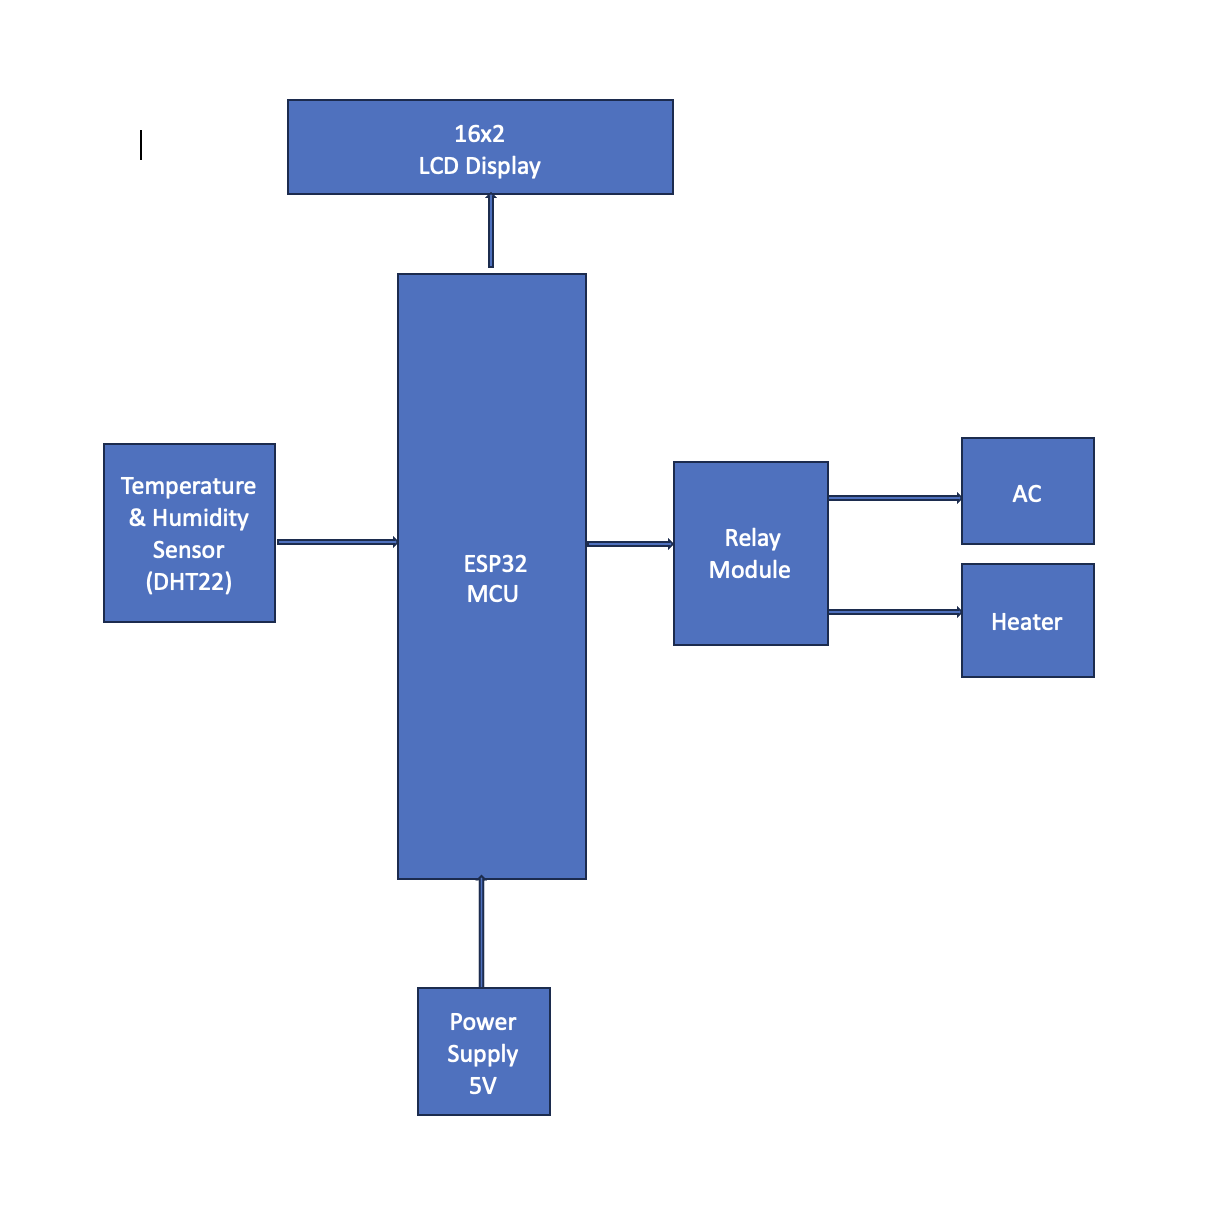
\includegraphics[width=0.6\textwidth]{BlockDiagram.png} % Replace with the actual block diagram image
    \caption{Block Diagram of the Smart Home Temperature and Humidity Monitoring System}
    \label{fig:blockdiagram}
\end{figure}

\section{List of Hardware Components}
The system utilizes the following hardware components:
\begin{itemize}
    \item \textbf{Microcontroller}: ESP32 (with integrated Wi-Fi for wireless communication).
    \item \textbf{Temperature and Humidity Sensor}: DHT22 sensor.
    \item \textbf{LCD Display}: 16x2 LCD to display real-time sensor data.
    \item \textbf{Relay Module}: Used to control the AC or heater.
    \item \textbf{Power Supply}: 5V regulated power supply.
\end{itemize}

\section{List of Software Components}
The software components required to run the system include:
\begin{itemize}
    \item \textbf{Embedded Code}: Written in C/C++ for controlling the ESP32 microcontroller and sensors.
    \item \textbf{Wi-Fi Communication Protocol}: HTTP or MQTT for communicating with the smartphone app.
    \item \textbf{User Interface}: Mobile app for displaying temperature and humidity data and allowing remote control of the system.
    \item \textbf{Sensor and Display Driver Code}: For reading sensor values and driving the LCD display.
\end{itemize}

\section{Flowchart/Algorithm}
The control logic for the system is explained in the flowchart (Figure~\ref{fig:flowchart}).

\begin{figure}[H]
    \centering
    \includegraphics[width=0.7\textwidth]{Flowchart.png} % Replace with the actual flowchart image
    \caption{Flowchart of System Control Logic}
    \label{fig:flowchart}
\end{figure}

\subsection*{Steps in Flowchart}
\begin{enumerate}
    \item \textbf{System Initialization:} Initialize all hardware components, including sensors (DHT22), the LCD screen, and the Wi-Fi module.
    \item \textbf{Read Sensor Data:} Read the temperature and humidity data from the DHT22 sensor.
    \item \textbf{Check Temperature:}
    \begin{itemize}
        \item If the temperature exceeds the preset upper threshold, turn on the air conditioner.
        \item If the temperature is below the lower threshold, turn on the heater.
        \item If the temperature is within the threshold range, no action is taken, and appliances remain off.
    \end{itemize}
    \item \textbf{Transmit Data:} Transmit collected data to a smartphone app via Wi-Fi and listen for control commands from the app.
    \item \textbf{Update Appliance Control:} Update appliance control based on user input or preset thresholds.
    \item \textbf{Loop Back:} Continuously loop back to read sensor data for real-time monitoring and control.
\end{enumerate}

\subsection*{Pseudocode}
\begin{verbatim}
BEGIN
    Initialize sensors, LCD, and Wi-Fi module
    Connect to Wi-Fi network
    WHILE system is active:
        Read temperature and humidity data from DHT22
        Display data on LCD
        IF temperature > upper threshold:
            Activate air conditioner
        ELSE IF temperature < lower threshold:
            Activate heater
        Transmit sensor data to the smartphone app
        Receive user input (if any) from smartphone app
        Adjust AC/heater control based on user input
    END WHILE
END
\end{verbatim}

\section{Communication Protocols}
The system uses the following communication protocols:
\begin{itemize}
    \item \textbf{I2C}: For communication between the ESP32 microcontroller and the LCD display.
    \item \textbf{Wi-Fi (HTTP/MQTT)}: To send temperature and humidity data to a smartphone app and receive control inputs remotely.
    \item \textbf{GPIO}: To control the relay module that activates the air conditioner or heater.
\end{itemize}

\section{Integration of Hardware and Software}
The hardware and software integration is achieved through the ESP32 microcontroller, which manages communication between the sensors, LCD, and the Wi-Fi module. The sensor data is collected and processed by the microcontroller, which then displays the information on the LCD and sends it via Wi-Fi to a smartphone app. Control signals from the app are processed by the microcontroller to switch appliances on or off through the relay module.

\section{Data Flow}
The system’s data flow involves:
\begin{enumerate}
    \item The DHT22 sensor continuously measures temperature and humidity.
    \item The ESP32 reads and processes this sensor data.
    \item Data is displayed on the LCD in real-time for local monitoring.
    \item The ESP32 sends the data via Wi-Fi to a smartphone app for remote monitoring.
    \item If the temperature exceeds or falls below predefined thresholds, the ESP32 activates the relay module to control the AC or heater.
    \item The smartphone app can override automatic controls by sending commands to the ESP32.
\end{enumerate}

\section{Future Improvements}
Potential future improvements include:
\begin{itemize}
    \item Integration with other smart home devices such as lights and window blinds.
    \item Adding machine learning algorithms to predict and optimize control based on user preferences.
    \item Extending the system to control multiple rooms or zones.
    \item Implementing energy-saving features such as solar power integration or efficient power management.
\end{itemize}

\section{Conclusion}
The Smart Home Temperature and Humidity Monitoring System effectively monitors and controls the indoor climate, ensuring comfort and energy efficiency. By integrating sensors, wireless communication, and automation, the system enhances quality of life in smart homes. Future expansions can make the system more versatile and sustainable, increasing its potential for adoption in modern settings.

\end{document}
